\documentclass{article}
\usepackage[utf8]{inputenc}
\usepackage[spanish]{babel}
\usepackage{listings}
\usepackage{graphicx}
\graphicspath{ {images/} }
\usepackage{cite}

\begin{document}

\begin{titlepage}
    \begin{center}
        \vspace*{1cm}
            
        \Huge
        \textbf{Parcial 1 Informática II}
            
        \vspace{0.5cm}
        \LARGE
        Informa2 S.A.S
            
        \vspace{1.5cm}
            
        \textbf{Johan David Rojas\\Luis Fernando Torres\\Mateo Alejandro Bravo}
            
        \vfill
            
        \vspace{0.8cm}
            
        \Large
        Despartamento de Ingeniería Electrónica y Telecomunicaciones\\
        Universidad de Antioquia\\
        Medellín\\
        Abril de 2021
            
    \end{center}
\end{titlepage}

\tableofcontents
\newpage
\section{Análisis del problema}\label{analisis}
Para solucionar este desafio, se plantea un algoritmos que esta dividido en 2 etapas.

\begin{itemize}
    \item \textbf{Etapa de Software}\label{sw}
    En esta etapa se recopila toda la información que el usuario ingresa por el monitor serial para ser procesada en la siguiente etapa. Aquí se debe ingresar el patrón de caracteres que el usuario desea ver en la matriz de LEDs y se realiza el proceso de llevar cada carecter a un sistema binario que la electronica del montaje entienda, es decir se codifica la solicitud del usuario.

    \item \textbf{Etapa de Hardware}\label{hw}
    En esta etapa se cuenta con un arreglo asignado para cada carácter. En el montaje del circuito se tiene ocho 74HC595 (cada uno controla una fila de la matriz) conectados de tal forma que llevándole información por el puerto SER mostrará un patrón correspondiente al carácter ingresado por el monitor serial. Cada posicion del arreglo nos dará información del dato a llevar al circuito integrado. Por cada circuito integrado habrá ocho salidas que en total serán 64 salidas que determinarán el estado de los LED, a cada LED se le conecta un resistor para evitar daños. 

\end{itemize}
Una vez explicadas las etapas que se van a tener en cuenta en la solución de este desafío, se comienza a analizar la manera en la que se debe realizar el procedimiento para mostrar un solo carácter en el arreglo de LEDs, es decir como se va a implementar la función Imagen(). Para ello se realiza una recopilación de ideas, con posibles pasos que debe llevar cada etapa y unas observaciones para tener muy claro que se hace, tal como se muestra en la figura(\textbf{\ref{f1}}) :

    \begin{figure}[h]
    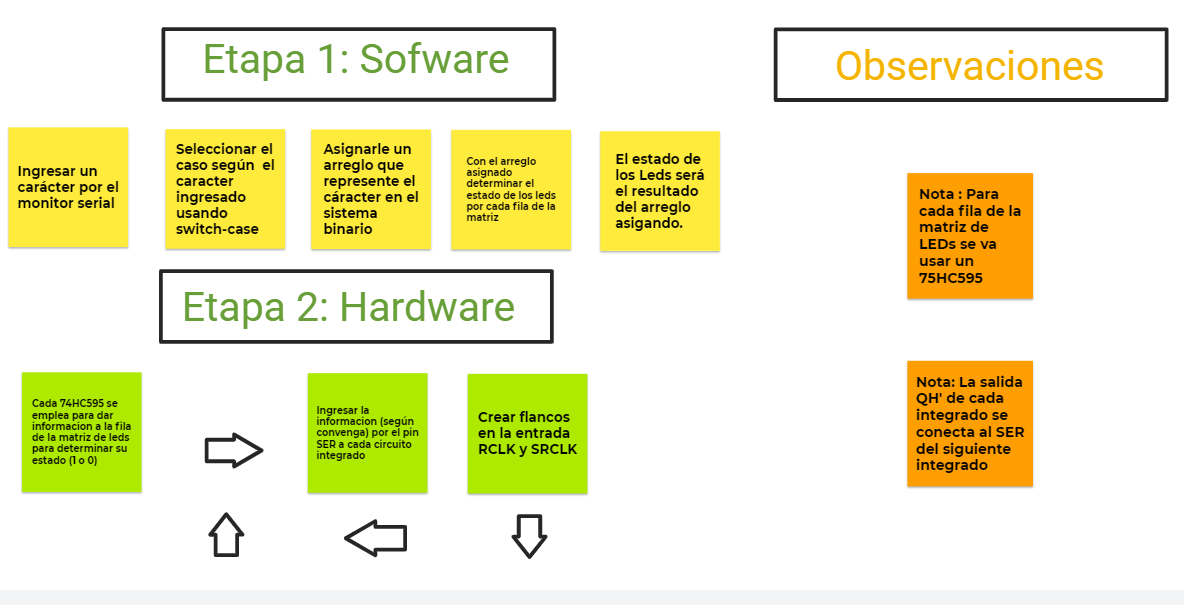
\includegraphics[width=12cm]{funimagen.png}
    \centering
    \caption{Procedimiento para mostrar un solo carácter}
    \label{f1}
    \end{figure}


\section{Desarrollo} \label{desarrollo}
Para llevar a cabo la solución de este reto, lo que se busca es que el carácter que la persona ingrese por el monitor serial, sea reflejado en una matriz de LEDs y que se pueda observar de manera clara. Para ello se debe utilizar el sistema binario, ya que este indica el estado de un LED, donde cero (0) representa apagado y el uno (1) encendido.\\

Teniendo en cuenta lo dicho anteriormente, lo que se va a hacer es mostrar el carácter ingresado, en un arreglo de números en  sistema binario, indicando que LEDs deben encenderse para formar dicho patrón ingresado en la matriz. tal como se muestre en la figura(\textbf{\ref{A}}):


    \begin{figure}[h]
    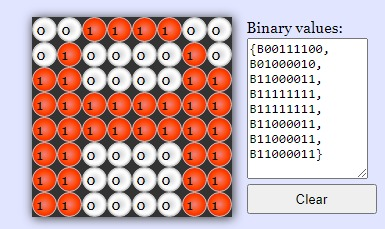
\includegraphics[width=8cm]{A.jpeg}
    \centering
    \caption{Letra A codificada para representar en la matriz}
    \label{A}
    \end{figure}

En la figura(\textbf{\ref{A}}), se puede observar el ejemplo con la letra A. En la matriz de LEDs que está ubicada en la parte izquierda, los números uno que están en color naranja, indican como se va a ver esta letra en la matriz real de LEDs. Por otra parte derecha muestra el arreglo que representa esta letra en sistema binario, el cual es el que se va a procesar por medio del integrado 74HC595. Para realizar este proceso de conversion se hizo uso de una herramineta online de mucha ayuda \cite{riyas}, la cual tiene como fin generar el arreglo en binario para ahorrar tiempo.\\

Después de obtener el arreglo en binario de toda la matriz, lo que se hace es separar cada fila, la cual está hecha con 8 LEDs, razón por la cual se debe formar subgrupos 8 bits  que indican el estado de cada fila. Al realizar esta acción, el arreglo queda con un tamaño de 8 posiciones donde cada espacio representa el estado de una fila de LEDs de la matriz. 



\bibliographystyle{IEEEtran}
\bibliography{references}

\end{document}
